\section{Consensus Distillation Is Design-Sensitive, Not Architecture-Limited}
\label{sec:distill}

The motivating gap for Track 2: \cmaj{} $b{=}5$ reaches $80\%$ on
dev (and $79\%$ on test, apples-to-apples) while greedy single-shot
\ctwo{} reaches $74\%$.  A $5\text{--}6$\,pp gap that scales
linearly in $b$ up to $b{=}5$ (saturated).  Track 2's question:
can a small commit-adapter LoRA close this gap by distilling
\cmaj{}'s consensus into a single forward pass?

This section reports two design iterations that fail (\ctwoc{} $=
70.5\%$ across $3.25\times$ capacity), a third design that succeeds
(\ctwoc{} $= 79.0\%$, within sampling error of the $80\%$ target),
and disentangling ablations that attribute the lift to where
commit fires in the diffusion schedule rather than to the
supervision signal.  The headline is that the v1/v2 plateau is a
\emph{design} bottleneck, not an architectural impossibility, and
the two design errors mask each other.

\subsection{The Plateau: v1 and v2 at \ctwoc{} $= 70.5\%$}
\label{subsec:distill_plateau}

The training data is \code{eren23/sfumato-commit-mixture-gsm8k} ---
$109$ rows derived from running \cmaj{} on $500$ GSM8K-train
problems and keeping three buckets ($46$ rescue, $58$
preserve-disagreement, $5$ pure-agreement; see \S\ref{sec:setup}).

\textbf{v1} uses target modules $[$\code{gate\_proj},
\code{up\_proj}, \code{down\_proj}$]$.  Of these only
\code{up\_proj} matches \LLaDA{}'s actual block, so the LoRA
attaches to $1/3$ of FFN, with $4.2$M trainable parameters.
\ctwoc{} $= 70.5\%$.

\textbf{v2} fixes the module-name bug: target modules
$[$\code{ff\_proj}, \code{up\_proj}, \code{ff\_out}$]$ --- the
\LLaDA{}-correct list, $3/3$ FFN match, $13.6$M trainable
parameters ($3.25\times$ v1).  Same data, same hyperparameters,
same answer-span loss, same last-block-only inference.
\ctwoc{} $= 70.5\%$.

The same $70.5\%$ across a $3.25\times$ capacity bump rules out a
capacity-limited reading: whatever is bottlenecking the adapter is
not parameter count.  A diagnostic comparison of decoded text with
\code{apply\_commit=True} versus \code{False} at $t{=}0$
(deterministic) on $10$ fixed problems confirmed this: text
shifts in $8$ of $10$ problems, but the answer never flips.  The
commit LoRA \emph{was} modifying tokens, but only late-block
tokens, which could not change the answer that earlier blocks had
already pinned.

\subsection{v3: Multi-Block Commit + Full-Response Loss}
\label{subsec:distill_v3}

Two design changes for v3, on the same $r{=}8$ FFN-only LoRA and
the same dataset:

\begin{enumerate}
    \item \textbf{Multi-block commit at inference}: enable the
          commit adapter on sub-blocks $2\text{--}4$ of $4$ (the
          trailing $75\%$ of the $128$-token generation), not just
          the last sub-block.  This corresponds to
          \code{COMMIT\_N\_BLOCKS=3} in the inference script.
    \item \textbf{Full-response training loss}: the
          masked-diffusion CE loss is computed over the entire
          response span \code{[prompt\_len, response\_end)}
          rather than the answer-tail span \code{[answer\_start,
          response\_end)}.  This corresponds to the
          \code{FULL\_RESPONSE\_LOSS=1} flag in the trainer.
\end{enumerate}

Both changes are inexpensive: the trainer adds a few lines, and
the inference change is a single integer flag.

Table~\ref{tab:distill_main} reports the headline numbers.

\begin{table}[h]
\centering
\caption{Track 2 commit-adapter results on GSM8K-test, $N{=}200$,
$k{=}64$, seed $0$.  v3 c2c $= 79.0\%$ is within sampling error of
the $80\%$ pre-registered target (binomial CI $\pm 5$\,pp at
$N{=}200$).  cmajc v2 $= 82.0\%$ on test is $+3$\,pp over base
test cmaj $= 79.0\%$.}
\label{tab:distill_main}
\smallskip
\begin{tabular}{lrr}
\toprule
Setup & \ctwoc{} & \cmajc{} \\
\midrule
Track 1 v2 alone (no commit) & $70.5\%$ & --- \\
+ commit v1 (last-block, answer-span) & $70.5\%$ & $81.5\%$ \\
+ commit v2 (last-block, answer-span) & $70.5\%$ & $\mathbf{82.0\%}$ \\
Track 1 v3 alone (no commit) & $73.0\%$ & --- \\
+ commit v3 ($n{=}3$, full-response) & $\mathbf{79.0\%}$ & $\mathbf{82.5\%}$ \\
\bottomrule
\end{tabular}
\smallskip\\
{\footnotesize\textit{$95\%$ CIs (Clopper--Pearson, $N{=}200$):}
Track 1 v2 alone \ctwoc{} \mbox{$[63.7, 76.7]$};
+commit v1 \ctwoc{} \mbox{$[63.7, 76.7]$}, \cmajc{} \mbox{$[75.4, 86.6]$};
+commit v2 \ctwoc{} \mbox{$[63.7, 76.7]$}, \cmajc{} \mbox{$[76.0, 87.1]$};
Track 1 v3 alone \ctwoc{} \mbox{$[66.3, 79.0]$};
+commit v3 \ctwoc{} \mbox{$[72.7, 84.4]$}, \cmajc{} \mbox{$[76.5, 87.5]$}.}
\end{table}

At $N{=}200$, the exact binomial $95\%$ CI for v3 \ctwoc{} is
$79.0\%$~\mbox{$[72.7, 84.4]$}, which contains the $80\%$
pre-registered target.  Track 2's pre-registered prediction \#1
(\ctwoc{} $\geq 80\%$) is therefore within CI of holding, with the
point estimate $+8.5$\,pp over the v1/v2 plateau.

\subsection{Disentangling: Block Coverage Versus Supervision}
\label{subsec:distill_ablations}

The v3 result bundles three changes from v2: full-FFN module
coverage on the upstream Track 1 LoRA (v2 $\to$ v3,
$+2.5$\,pp on no-prefix \ctwo{}), $n_\text{blocks}$ $1 \to 3$ on
inference, and answer-span $\to$ full-response on training.
We disentangle the second two with two ablations on the same
Track 1 v3 base, holding everything else fixed.

\begin{table}[h]
\centering
\caption{Disentangling ablations.  Block coverage
($n_\text{blocks}{=}3$) drives most of the lift.  Full-response
loss adds $+2.0$\,pp on top, but on its own (with
$n_\text{blocks}{=}1$) adds nothing.  The two design errors mask
each other.}
\label{tab:distill_disentangle}
\smallskip
\begin{tabular}{llllrr}
\toprule
Setup & LoRA & commit & $n_\text{blocks}$ & training loss & \ctwoc{} / $\Delta$ \\
\midrule
Track 1 v3 alone & v3 & --- & --- & --- & $73.0\%$ / --- \\
\textbf{ABL\_A} & v3 & v2 & $\mathbf{3}$ & answer-span & $\mathbf{77.0\%}$ / $\mathbf{+4.0}$ \\
\textbf{ABL\_B} & v3 & v3 & $1$ & full-response & $73.0\%$ / $+0.0$ \\
\textbf{v3 full} & v3 & v3 & $\mathbf{3}$ & full-response & $\mathbf{79.0\%}$ / $\mathbf{+6.0}$ \\
\bottomrule
\end{tabular}
\smallskip\\
{\footnotesize\textit{$95\%$ CIs (Clopper--Pearson, $N{=}200$):}
Track 1 v3 alone \mbox{$[66.3, 79.0]$};
\textbf{ABL\_A} \mbox{$[70.5, 82.6]$};
\textbf{ABL\_B} \mbox{$[66.3, 79.0]$};
\textbf{v3 full} \mbox{$[72.7, 84.4]$}.  CIs on the
\textbf{ABL\_A} vs.\ \textbf{v3 full} difference ($+2$\,pp on
top of multi-block commit) and the \textbf{ABL\_B} vs.\ Track 1
v3 alone non-difference are paired-sample quantities; per-problem
JSONLs released alongside the adapters support paired analysis.}
\end{table}

\textbf{Block coverage ($n_\text{blocks}{=}3$) is the dominant
driver}: $+4.0$\,pp on its own, even with the sub-optimal v2
answer-span supervision (ABL\_A).
\textbf{Full-response loss alone}: $+0.0$\,pp (ABL\_B).
Full-response training has \emph{no leverage} if commit application
is still gated to the last sub-block.
\textbf{Combination}: $+6.0$\,pp.  Full-response loss adds
$+2.0$\,pp on top of multi-block commit.

The two design errors mask each other.  Late-block-only commit is
a structural bottleneck that prevents the supervision change from
doing any work, and answer-span-only training is a supervision
bottleneck that prevents the structural change from doing all of
its work.  The cleanest one-sentence statement: \emph{once commit
fires earlier in the diffusion schedule, even sub-optimal
supervision recovers most of the value}.

The \textbf{ABL\_B} null result is consistent with the mechanism
story we develop in \S\ref{subsec:distill_mechanism}; a sanity
probe verifying the v3 adapter loads and modifies inference at
the \texttt{COMMIT\_N\_BLOCKS=1} configuration is deferred
(\appref{app:open}).

\begin{figure}[t]
\centering
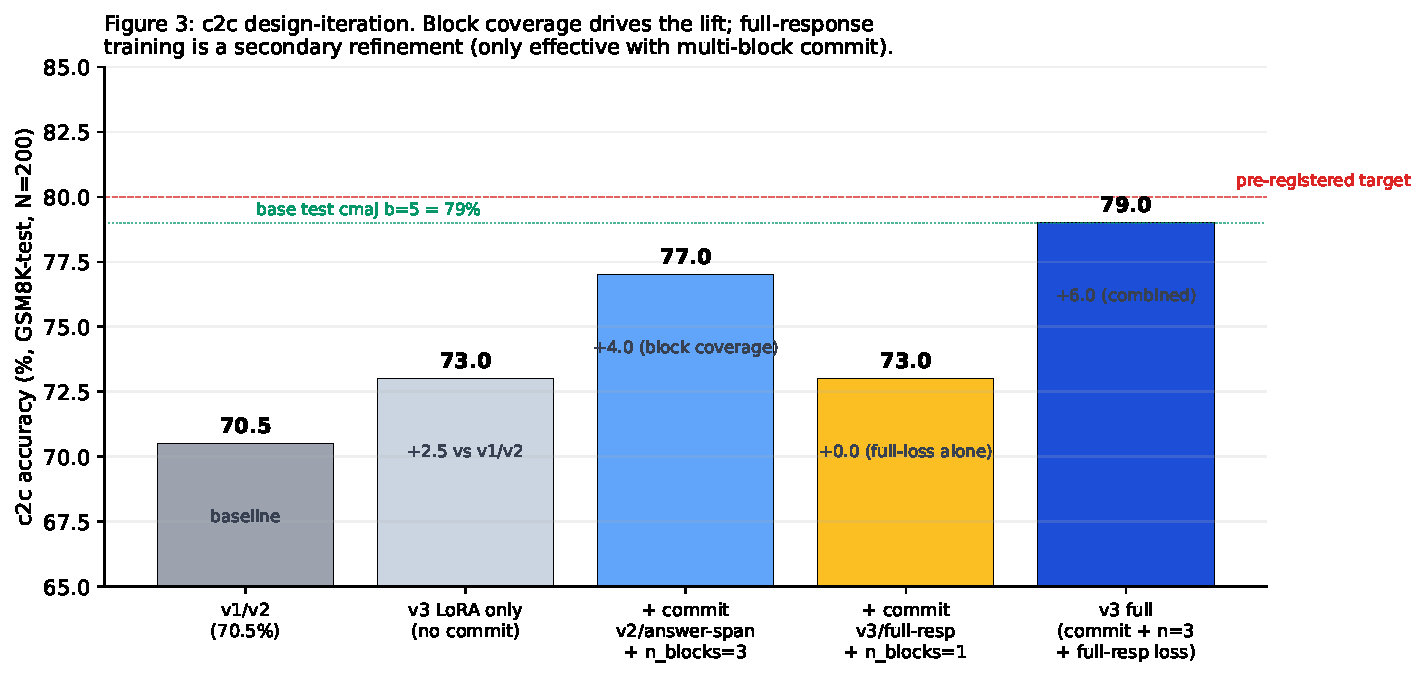
\includegraphics[width=\textwidth]{figures/fig3_c2c_design_iteration.pdf}
\caption{c2c design-iteration disentangling.  Five bars: v1/v2
baseline, v3 LoRA alone, ABL\_A (block coverage with v2
answer-span supervision), ABL\_B (full-response loss with
last-block-only commit), v3 full.  The pre-registered $80\%$
target and base test \cmaj{} of $79\%$ lines are visible.  The
$+0.0$ result for ABL\_B (full-response loss with
$n_\text{blocks}{=}1$) makes the ``block coverage is dominant''
story visually unambiguous.  Generated by
\code{scripts/make\_paper\_figures.py}.}
\label{fig:c2c_design}
\end{figure}

\subsection{Mechanism}
\label{subsec:distill_mechanism}

\textbf{The 96-token prefix problem.}  \LLaDA{}'s semi-AR sampler
generates $128$ tokens in $4$ sub-blocks of $32$.  By the time the
sampler reaches the last sub-block, the previous $96$ tokens have
committed the chain-of-thought, and the answer is largely implied
by the reasoning that has already been laid down.  A commit-LoRA
that fires \emph{only} on the last sub-block can shift the
literal answer-tokens, but those tokens are downstream of the
reasoning that already determined the answer.  The diagnostic
$8/10$ text-shift, $0/10$ answer-flip result
(\S\ref{subsec:distill_plateau}) is exactly this picture.

When commit fires on sub-blocks $2$--$4$, the LoRA can shape the
\emph{trajectory} of the late CoT, not just the answer literal.
Once the trajectory is malleable, the answer-token shift becomes
load-bearing because the answer-tokens are now downstream of a
trajectory the adapter helped produce.

Full-response training reinforces this.  An answer-span-only loss
teaches the LoRA to predict the answer given a fixed CoT context,
which is approximately what the base model already does.  A
full-response loss teaches the LoRA to predict the entire
trajectory of consensus-quality reasoning, which is the harder
task and the one that generalizes when commit is applied to
mid-trajectory blocks.  The \textbf{ABL\_B} null result
(Table~\ref{tab:distill_disentangle}, $+0.0$\,pp from full-response
training when commit fires only on the last sub-block) is the
cleanest empirical signature of this mechanism: even better
supervision cannot rescue surgery whose temporal placement is
wrong.

\subsection{Compositionality with Branch Aggregation}
\label{subsec:distill_compose}

Pre-registered prediction \#3 was that \cmajc{} (\cmaj{} with
commit-LoRA per branch) would not exceed \cmaj{} $b{=}5$ by more
than $1$\,pp --- the intuition being that if commit-LoRA is doing
useful work, that work should already be captured by majority vote
across stochastic branches, and stacking should produce no
double-dip.

The result with commit v2: \cmajc{} $= 82.0\%$~\mbox{$[76.0, 87.1]$}
on test versus base test \cmaj{} $= 79.0\%$~\mbox{$[72.7, 84.4]$},
a $+3$\,pp delta.  The result with commit v3 (the c2c-fixed
design, \code{COMMIT\_N\_BLOCKS=3}, full-response training):
\cmajc{} $= 82.5\%$~\mbox{$[76.5, 87.5]$}, a $+3.5$\,pp delta over
base test \cmaj{}.  Pre-reg violated upward in both cases.  Branch
aggregation and weight-space commit do partially independent work,
and the gains compose under both Track 2 designs.

\textbf{Branch aggregation absorbs much of the structural
correction that the v3 commit delivers in single-pass inference.}
Commit v3 beats commit v2 by $+8.5$\,pp on the single-pass
\ctwoc{} setting ($79.0\%$ vs $70.5\%$) but matches it
statistically on the branch-aggregated \cmajc{} setting ($82.5\%$
vs $82.0\%$, both within each other's CI at $N{=}200$).
Figure~\ref{fig:b1_vs_b5} visualizes the collapse.

\begin{figure}[t]
\centering
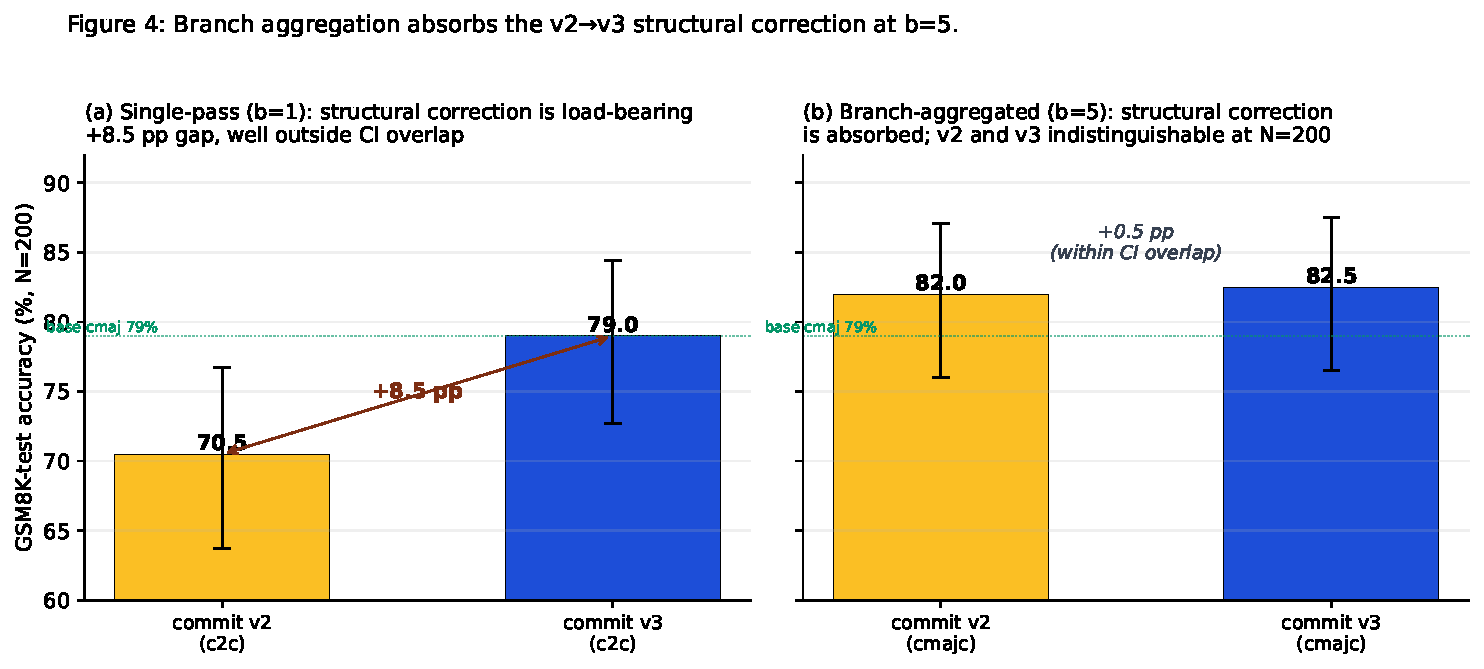
\includegraphics[width=\textwidth]{figures/fig4_b1_vs_b5_collapse.pdf}
\caption{Branch aggregation absorbs the v2$\to$v3 structural
correction.  At $b{=}1$ (left), the structurally-correct v3
commit beats the structurally-incorrect v2 commit by $+8.5$\,pp,
well outside CI overlap.  At $b{=}5$ (right), the same two
adapters are statistically indistinguishable.  Stochastic
branch-vote already recovers the consensus quality that the
late-block-only v2 commit misses, leaving the v3 commit's
structural advantage with little incremental room to operate.
Generated by \code{scripts/make\_paper\_figures.py}.}
\label{fig:b1_vs_b5}
\end{figure}  The
mechanistic reading: \cmaj{} selects among trajectories sampled
at temperature; commit-LoRA biases each individual trajectory
toward consensus-quality reasoning before voting.  At $b{=}5$,
branch aggregation already recovers much of the consensus quality
that the late-block-only commit (v2) misses, so additional
structural correction at the per-trajectory level (v3) has less
incremental room to operate.  The implication for distillation
practice: where the v3 commit's marginal contribution is largest
is exactly where it is most needed --- at $b{=}1$.  For
single-pass inference, the structurally-correct design pays;
under stochastic-aggregation regimes, the structurally-incorrect
design is indistinguishable.

\paragraph{Status.}
\cmajc{} on the v3 commit was added in this revision and reaches
$82.5\%$~\mbox{$[76.5, 87.5]$}; the cmajc-v2 number ($82.0\%$)
remains in Table~\ref{tab:distill_main} for the historical
record.  The two are statistically indistinguishable at $N{=}200$.
